\section{La sililformilazione di alchini e la desililazione}

\diapo{Idrosililazione di alchini}
L'{\bf idrosililazione} di alchini terminali catalizzata da acido cloroplatinico è {\bf regioselettiva e diastereoselettiva} come mostrato in figura.
\begin{figure}{\centering{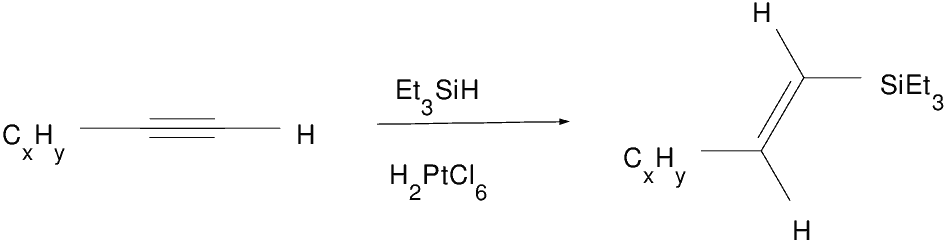
\includegraphics[width=0.80\textwidth]{img/sintesi/idro2.png}}}\end{figure}


\end{frame}

%%%%%%%%%%%%%%%%%%%%%%%%%%%%%%%%%%%%%%%%%%%%%%%%%%%%%%%%%%%%%%%%%%%%ho 


\diapo{Sililformilazione di alchini}
La {\bf sililformilazione} avviene in {\bf atmosfera di CO} e con catalizzatori a base di {\bf rodio}. 

Il {\bf silicio attacca l'atomo terminale} mentre il CO attacca il carbonio interno dando un'aldeide, come mostrato in alto nella figura.
\begin{columns}
\column{0.5\linewidth}
\begin{figure}{\centering{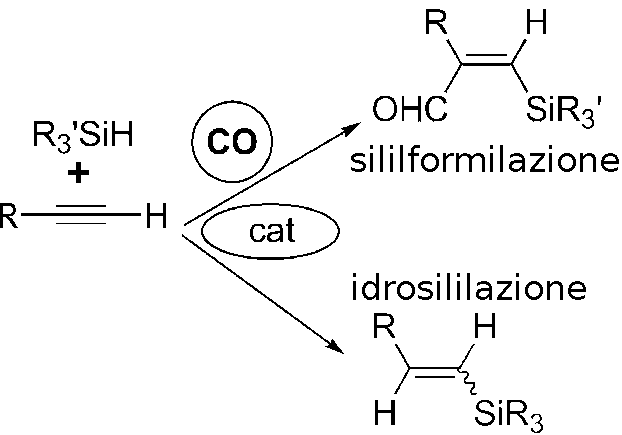
\includegraphics[width=1\textwidth]{img/sintesi/byproducts.png}}}\end{figure}
\pause
\column{0.5\linewidth} 

{\bf Se R è ingombrato} il prodotto di sililformilazione si forma {\bf più difficilmente} mentre è favorito il {\bf sottoprodotto di idrosililazione}.
\end{columns}

\end{frame}

\subsubsection{Idrosilani}\begin{frame}\frametitle{Sililformilazione di alchini}\framesubtitle{Idrosilani}
\begin{columns}
\column{0.35\linewidth}I {\bf sostituenti} sul reagente {\bf idrosilano} sono {\bf importanti} per il successo della reazione. 
\column{0.65\linewidth}\begin{figure}{\centering{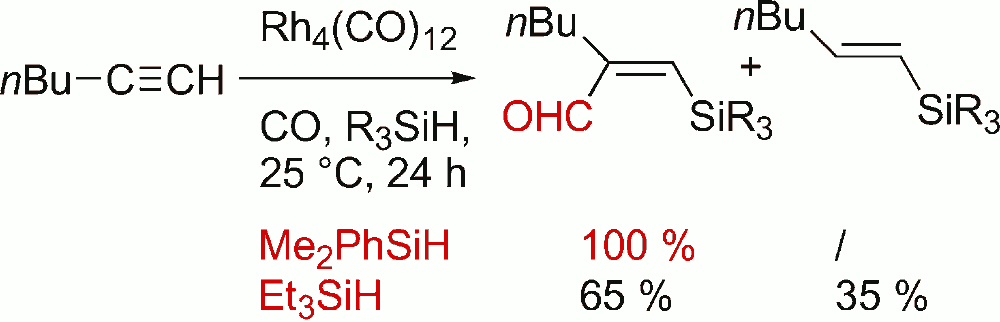
\includegraphics[width=1\textwidth]{img/sintesi/idrosilani.png}}}\end{figure}
\end{columns}\vspace{10pt}
La presenza di un sostituente {\bf aromatico favorisce} la sililformilazione rispetto all'idrosiliazione.

Sono {\bf preferibili} sostituenti aromatici con {\bf piccolo ingombro sterico}. 

\end{frame}

%%%%%%%%%%%%%%%%%%%%%%%%%%%%%%%%%%%%%%%%%%%%%%%%%%%%%%%%%%%%%%%%%%%%

\diapo{Sililcarbociclizzazione di ammine ed alcoli propargilici}
In presenza di un {\bf gruppo alcolico o di una ammide in posizione propargilica} ed impiegando una {\bf base} in quantità catalitica è possibile ottenere {\bf sililcarbociclizzazione}. 
\pause
\begin{figure}{\centering{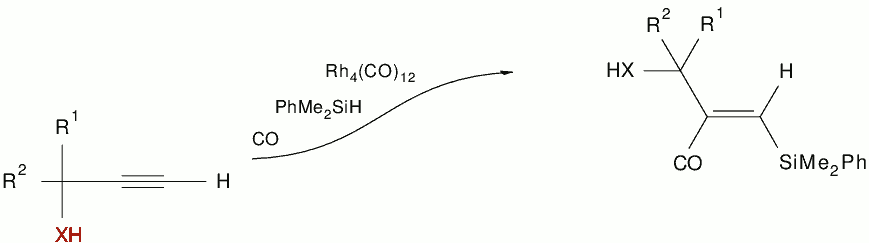
\includegraphics[width=0.6\textwidth]{img/sintesi/ciclizzaz-x1.png}}}\end{figure}
\pause
\vskip -30pt
\begin{figure}{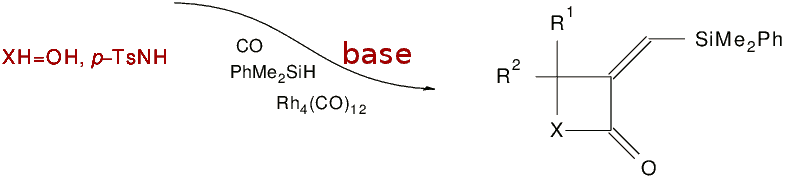
\includegraphics[width=0.75\textwidth]{img/sintesi/ciclizzaz-x2.png}}\end{figure}
\pause
Questa reattività è {\bf favorita da idrosilani con aromatici ingombrati e da \ce{R^1} e \ce{R^2} stericamente ingombranti}.

\end{frame}

%%%%%%%%%%%%%%%%%%%%%%%%%%%%%%%%%%%%%%%%%%%%%%%%%%%%%%%%%%%%%%%%%%%%
\logo{}
\diapo{Desililazione con migrazione del gruppo aromatico}

Tra tutte le numerose possibili ulteriori trasformazioni verrà esposta solamente la {\bf desililazione promossa da fluoruri con migrazione del gruppo aromatico} presente sull'idrosilano.  
\begin{figure}{\centering{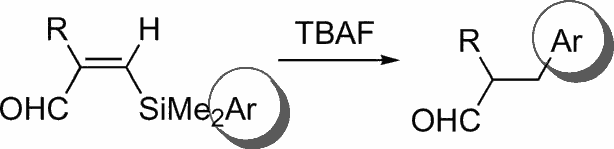
\includegraphics[width=0.5\textwidth]{img/sintesi/trasf_aromatico.png}}}\end{figure}
\pause
\begin{columns}
\column{0.8\linewidth}Inizialmente avviene l'{\bf attacco del fluoruro sull'atomo di silicio} rendendolo pentavalente. 
\pause

 Poi si ha una {\bf migrazione 1,2 anionotropica} del gruppo aromatico 
con ritenzione della configurazione originale anche in presenza di sostituenti in orto.
\column{0.3\linewidth}
\vskip -5pt
\begin{figure}{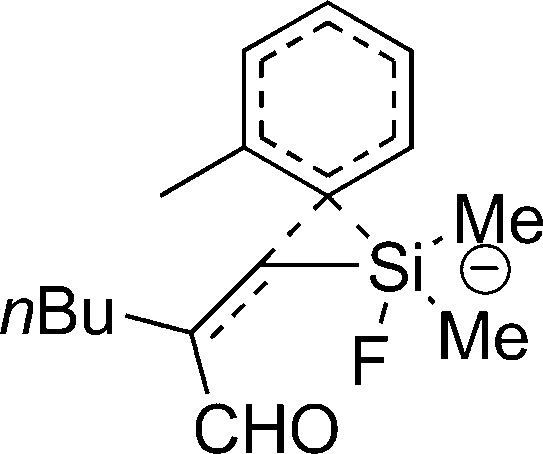
\includegraphics[width=1\textwidth]{img/sintesi/trasposizione12.png}}\end{figure}
\end{columns}
\end{frame}

%%%%%%%%%%%%%%%%%%%%%%%%%%%%%%%%%%%%%%%%%%%%%%%%%%%%%%%%%%%%%%%%%%%%

\begin{frame}\frametitle{Desililazione con migrazione del gruppo aromatico}
\begin{columns}
\column{0.5\linewidth}
Successivamente alla trasposizione 1,2 anionotropica dell'aromatico si ha una {\bf trasposizione [1,4]Si da carbonio ad ossigeno} detta ``riarrangiamento di Brook''. 

{\onslide<2>

La \emph{driving force} di questa reazione è la {\bf differenza di energia di legame Si-C e Si-O}. 

Infine il sililetere viene {\bf idrolizzato ad aldeide}.}

\column{0.5\linewidth}{\onslide<1,2>\begin{figure}{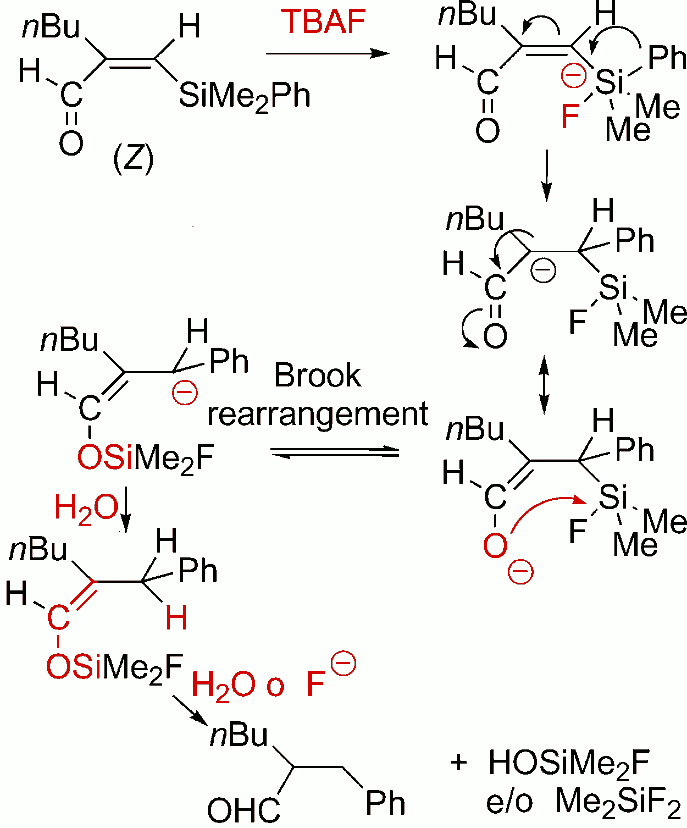
\includegraphics[width=1\textwidth]{img/sintesi/desililaz.png}}\end{figure}}
\end{columns}


\end{frame}

\logo{
\includegraphics[width=0.07\paperwidth]{img/snslogo.png}}
